\section{Distributed Octrees}

In this section we describe our software for the creation of octrees for the kiFMM in $\mathbb{R}^3$, Bempp-Tree\footnote{https://github.com/bempp/bempp-rs/tree/main/tree}. We've re-implemented optimal algorithms for the `bottom-up' construction of trees in parallel, whereby points distributed across each node are assembled into a parallel tree partitioned and load-balanced across a distributed system \cite{sundar2008bottom}. We demonstrate that on a single-node, our tree software performs well in comparison to leading single-node FMM codes \cite{wang2021exafmm}, where parallel experiments are omitted due to time constraints. In addition to good scaling, we leverage the power of Rust's Traits to write software that generalises across single-node and multi-node trees, allowing for users to implement single/multi-node fast algorithms with relative ease. We begin by describing in detail our method for constructing trees, following the discussion in \cite{sundar2008bottom}. A significant point of departure is how they achieve a 2:1 balancing scheme, which is essential for achieving the complexity bound in adaptive FMM implementations. We conclude with a short discussion on the communication intensive phases of the FMM in a distributed-memory FMM implementation, and how these can be addressed, as the next stage of this research project centers on the construction of a distributed memory kiFMM.

Beginning with the construction of uniform single-node trees.

- Algorithm for construction of uniform trees.
- why is bottom up construction a good idea?


Adaptive trees require balancing to ensure that we maintain the algorithmic complexity of the FMM.

- how do approaches to balancing differ between types of tree?
- in bottom up trees, we require 2 global sorts when balancing. This becomes a bottleneck. How do we address this? Offer a complexity, and reference software that already implements this.
- this is the first instance of communicatation bottleneck for the FMM.

Figure \ref{fig:chpt:3:sec:0:single_node_scaling} shows scaling of our software, `Bempp-Tree', on a single node ...

- what causes a significant constant difference between adaptive and uniform trees?

\begin{figure}[h]
  \centering
  \begin{minipage}[b]{0.45\textwidth}
    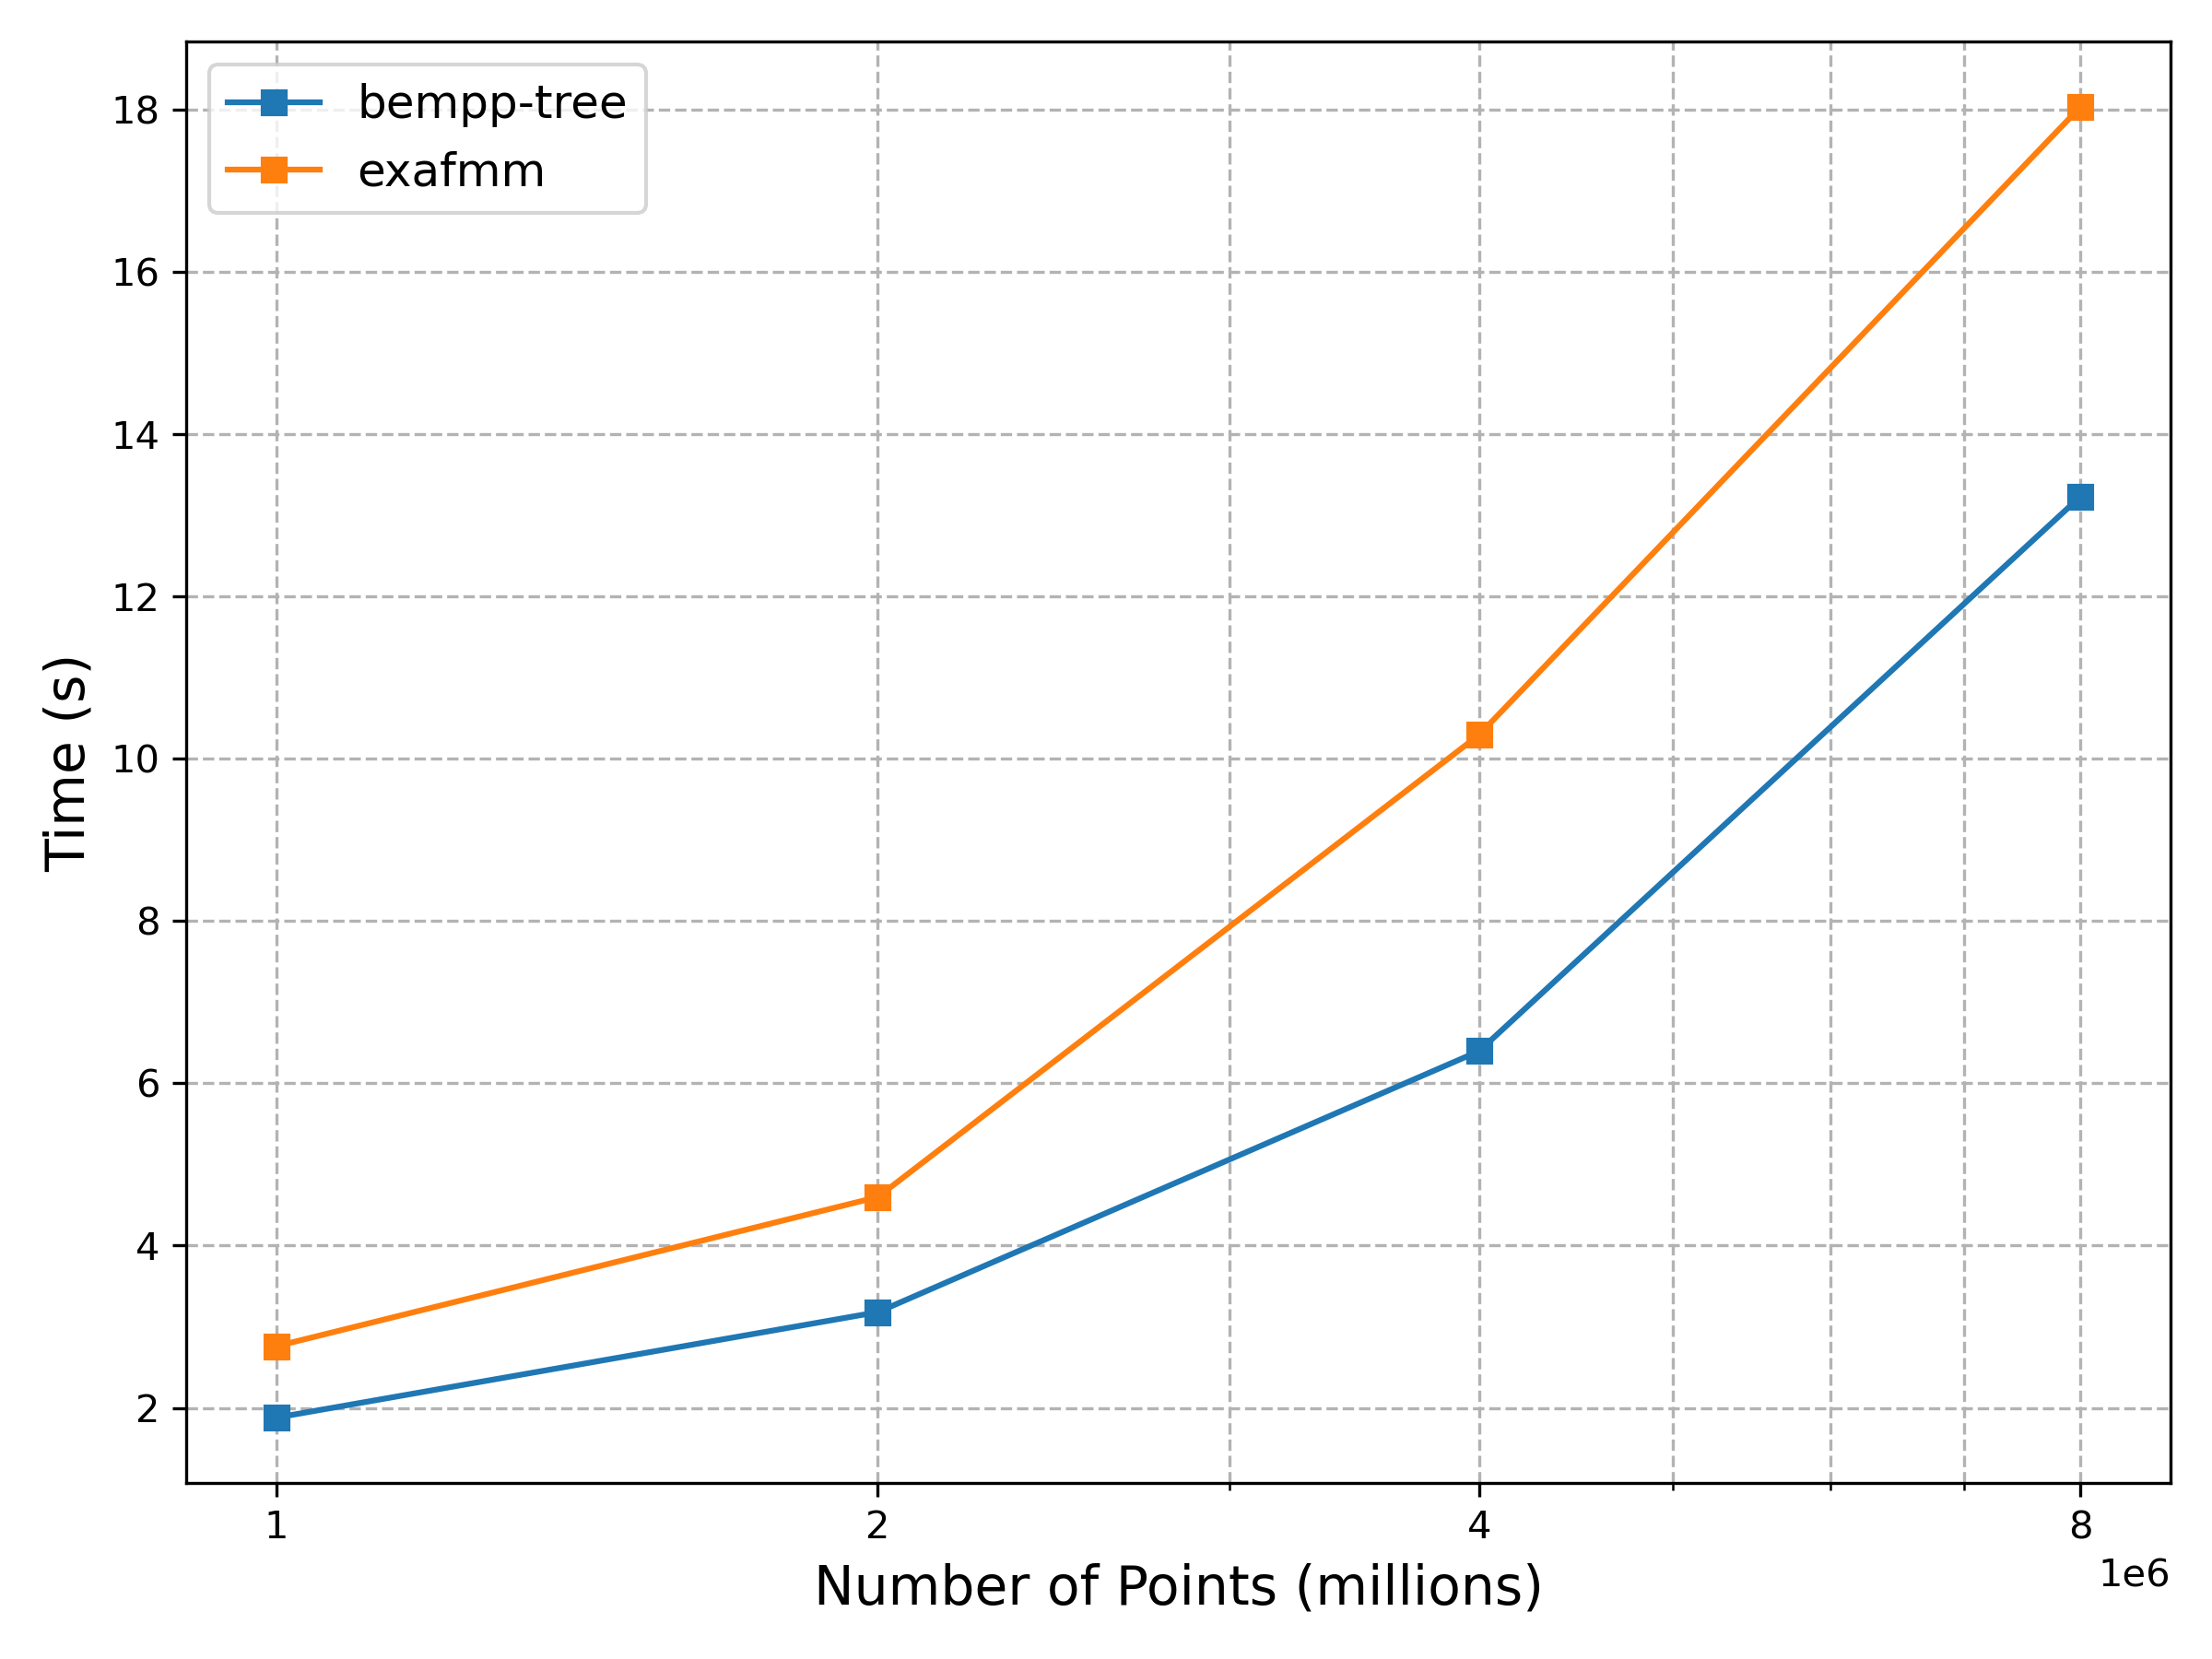
\includegraphics[width=\textwidth]{images/ch_3/single_node_scaling.png}
  \end{minipage}
  \hfill
  \begin{minipage}[b]{0.45\textwidth}
    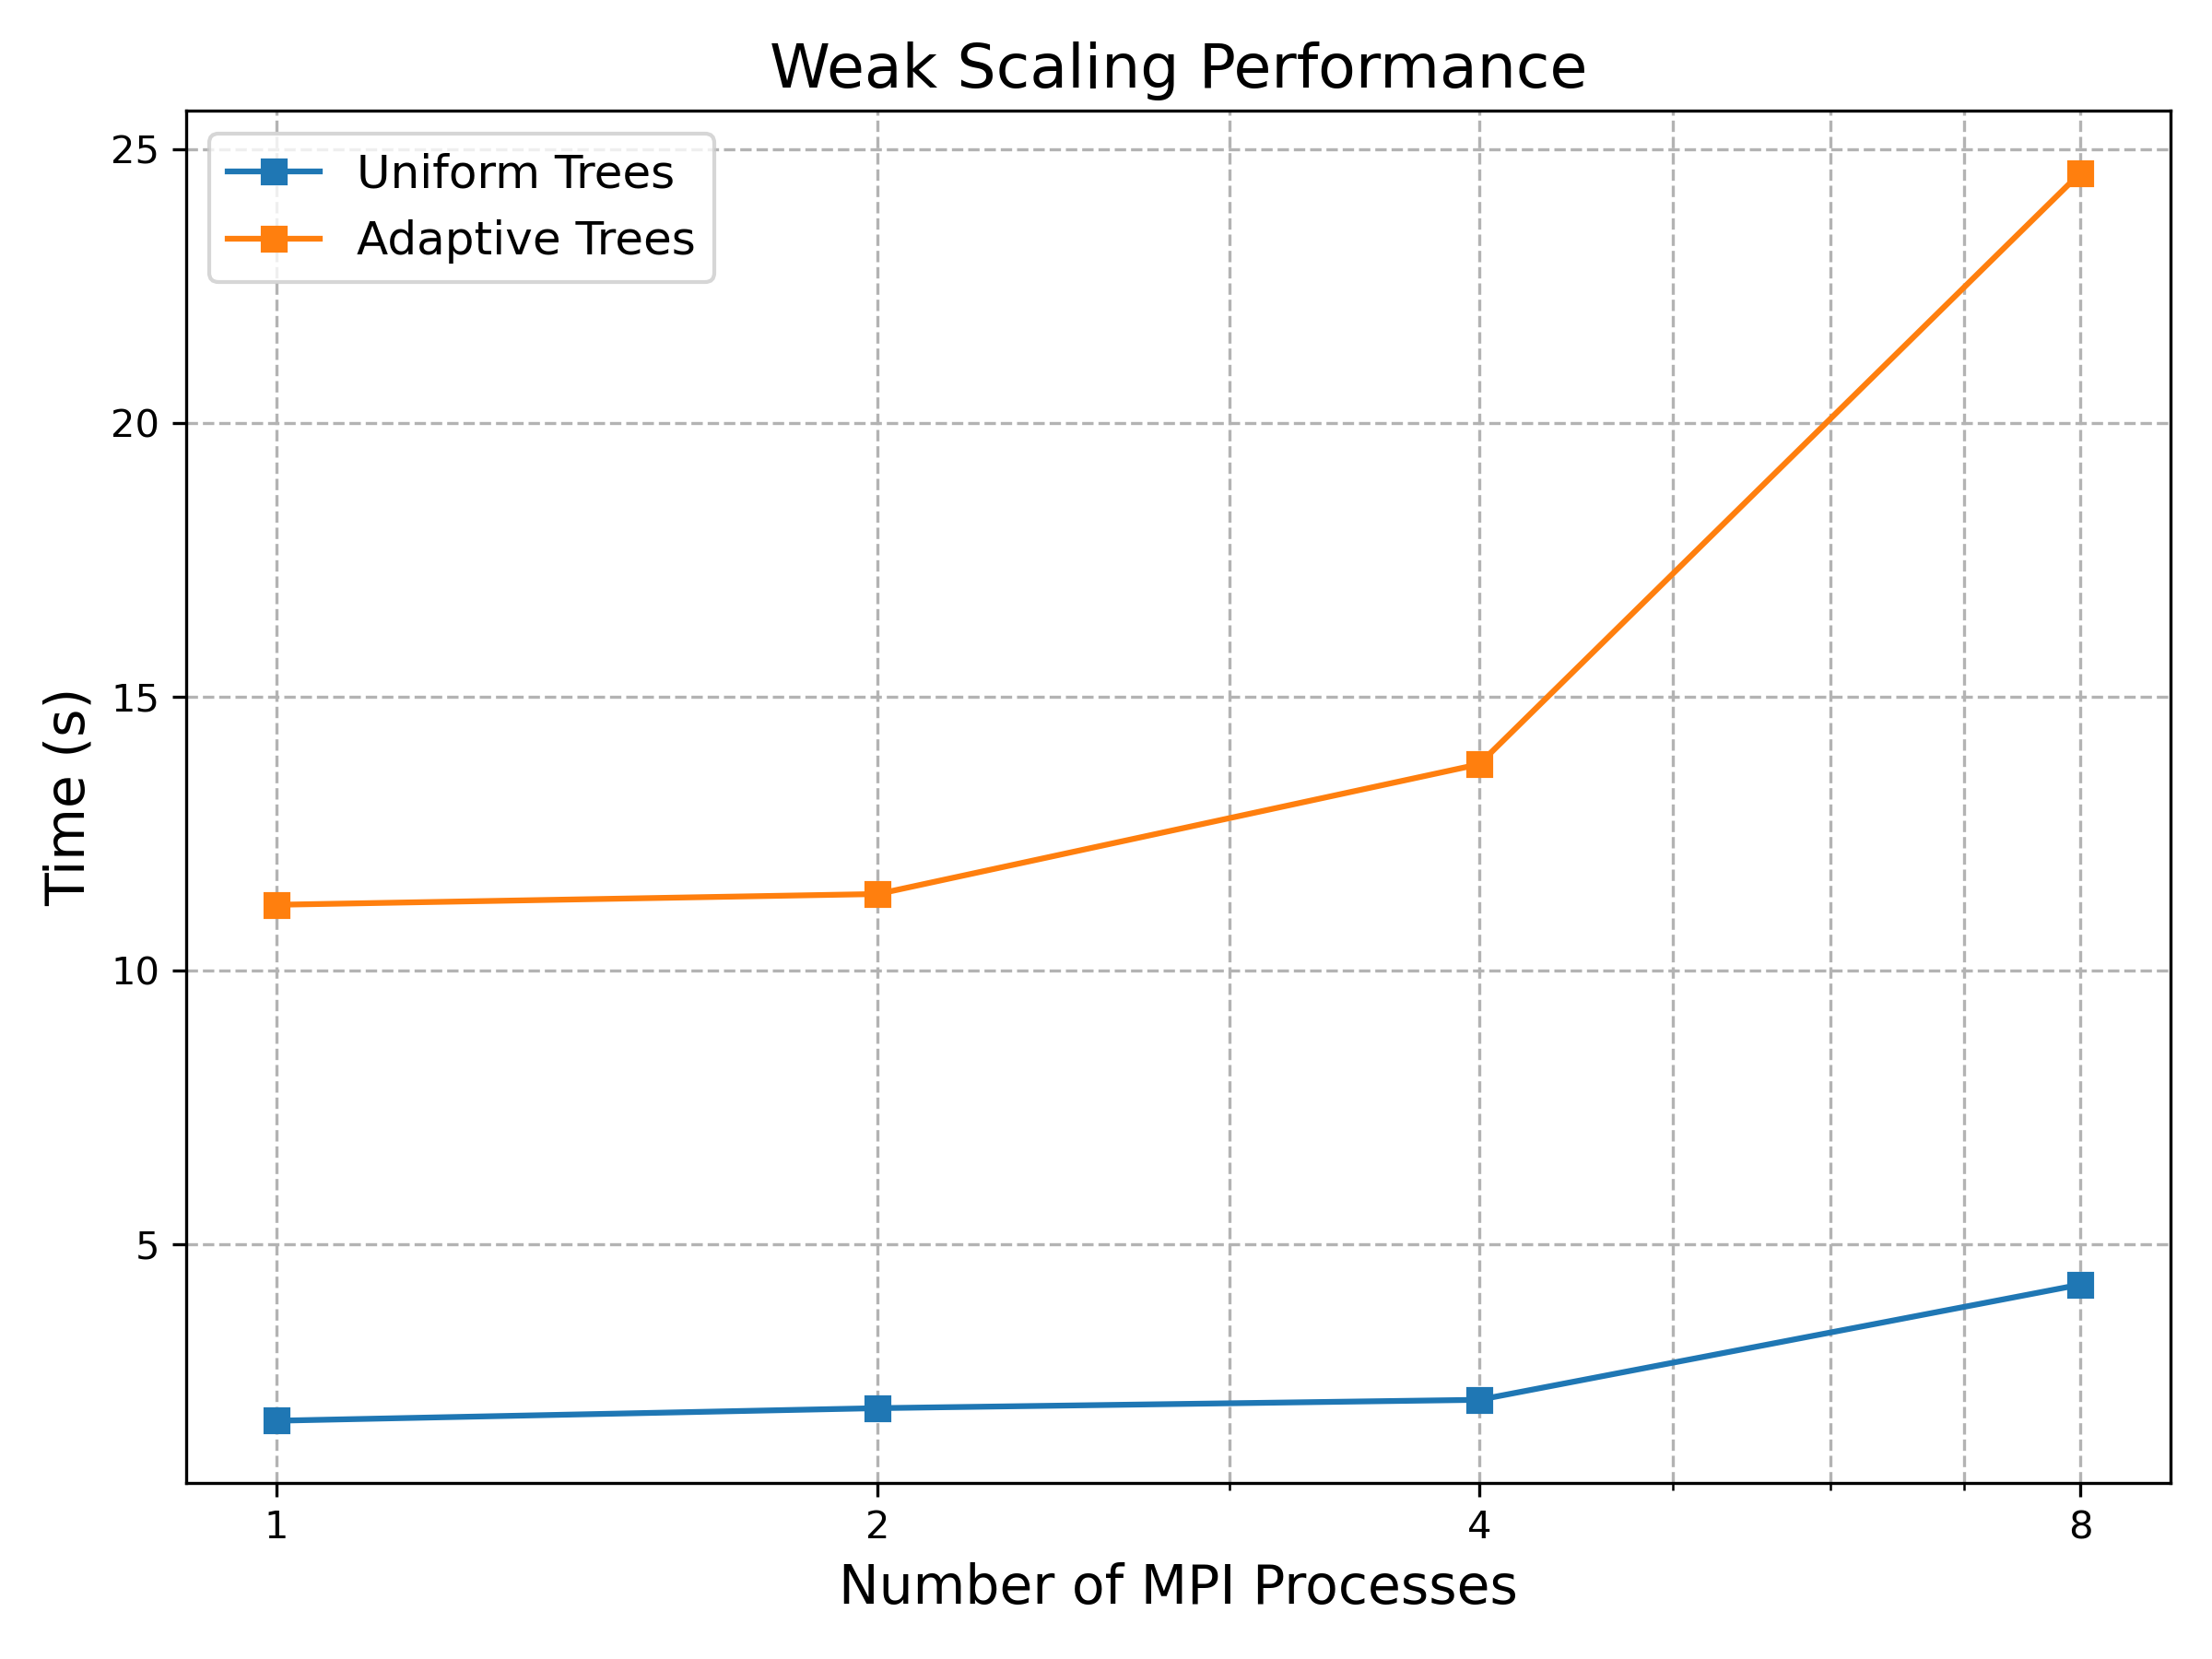
\includegraphics[width=\textwidth]{images/ch_3/weak_scaling_graph.png}
  \end{minipage}
\caption{The left figure shows the runtime of creating uniform trees on a single node in Bempp-Tree, in comparison to ExaFMM-T. The right figure shows weak scaling (over cores on a single node) of creating uniform and adaptive trees with Bempp-Tree, where each core is given 1e6 points. The uniform trees are partitioned to a depth of 5, the adaptive trees have at most 150 particles in their leaf boxes.}
\label{fig:chpt:3:sec:0:single_node_scaling}
\end{figure}


The second instance of a communication bottleneck in the FMM is during the evaluation of of $T^{M2M}$ and $T^{M2L}$.

- What is a locally essential tree? What are the communication intensive parts in its creation?

- How must we break down the communication pattern during this algorithm to achieve optimal communication bound of the FMM? (global vs local tree)?

